\documentclass[a4paper,11pt]{article} 
\usepackage{graphicx}

\begin{document}

\title{\sf 3DIR spectroscopy of water}
\author{GR0: F. Rao, D. Prada-Gracia}
\date{\today}
\maketitle

\section{Introduction}

This is a good example for a figure citations.
As shown in Fig.~\ref{mydata}, we were right! 
Below you see how to create a new paragraph.

Lorem ipsum dolor sit amet, pri ne delectus
salutandi accusamus, nec ut ullum dicit eirmod. Unum vero theophrastus no est,
mel in dicant homero consequat. Ad nam aeterno nominati argumentum. Eos id sint
congue deleniti, qui ad homero nostrum. Ut eam perfecto omittantur, nam
apeirian tractatos in, te cum doming commodo vidisse.

\begin{figure}
\centering
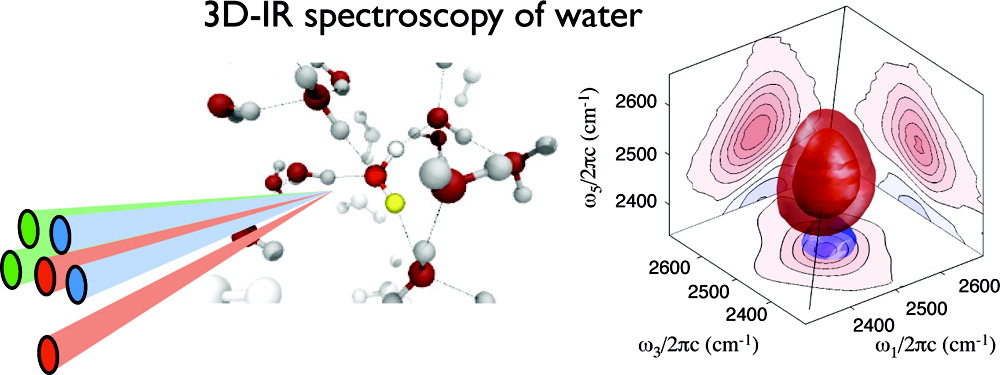
\includegraphics[width=100mm]{myfig}
\caption{Put here a description of the figure}
\label{mydata}
\end{figure}

You can even write equations:
\begin{equation}
y= ax+c - \sum_i x^i
\end{equation}
No vim suas quando. Quem sadipscing ut cum, ex ius mentitum verterem, consul
petentium nam ei. No ius quando homero. Agam sanctus eu vis, tota dictas sit
ea. Te vis audiam labores, pri at stet eligendi appellantur. In duis dolorem
eos.

A second equatio here (note the numbering automatic changed):
\begin{equation}
E=mc^2
\end{equation}


\end{document}
